\section{Design and Implementation}

\subsection{Hardware Design}


\subsubsection{Waist}
The base of the arm (or waist) was placed on a rotating platform at the front of Tiberius.  This controls the azimuthal angle of the arm, to allow it to position itself to the homed position, the active position or to move to face the direction of the object.  A large stepper motor is used to turn a corrugated rubber belt which turns a large base cog which was custom made using 3D printing.  This rotates the whole arm through the desired angle.

\begin{figure}[!htb]
\begin{center}
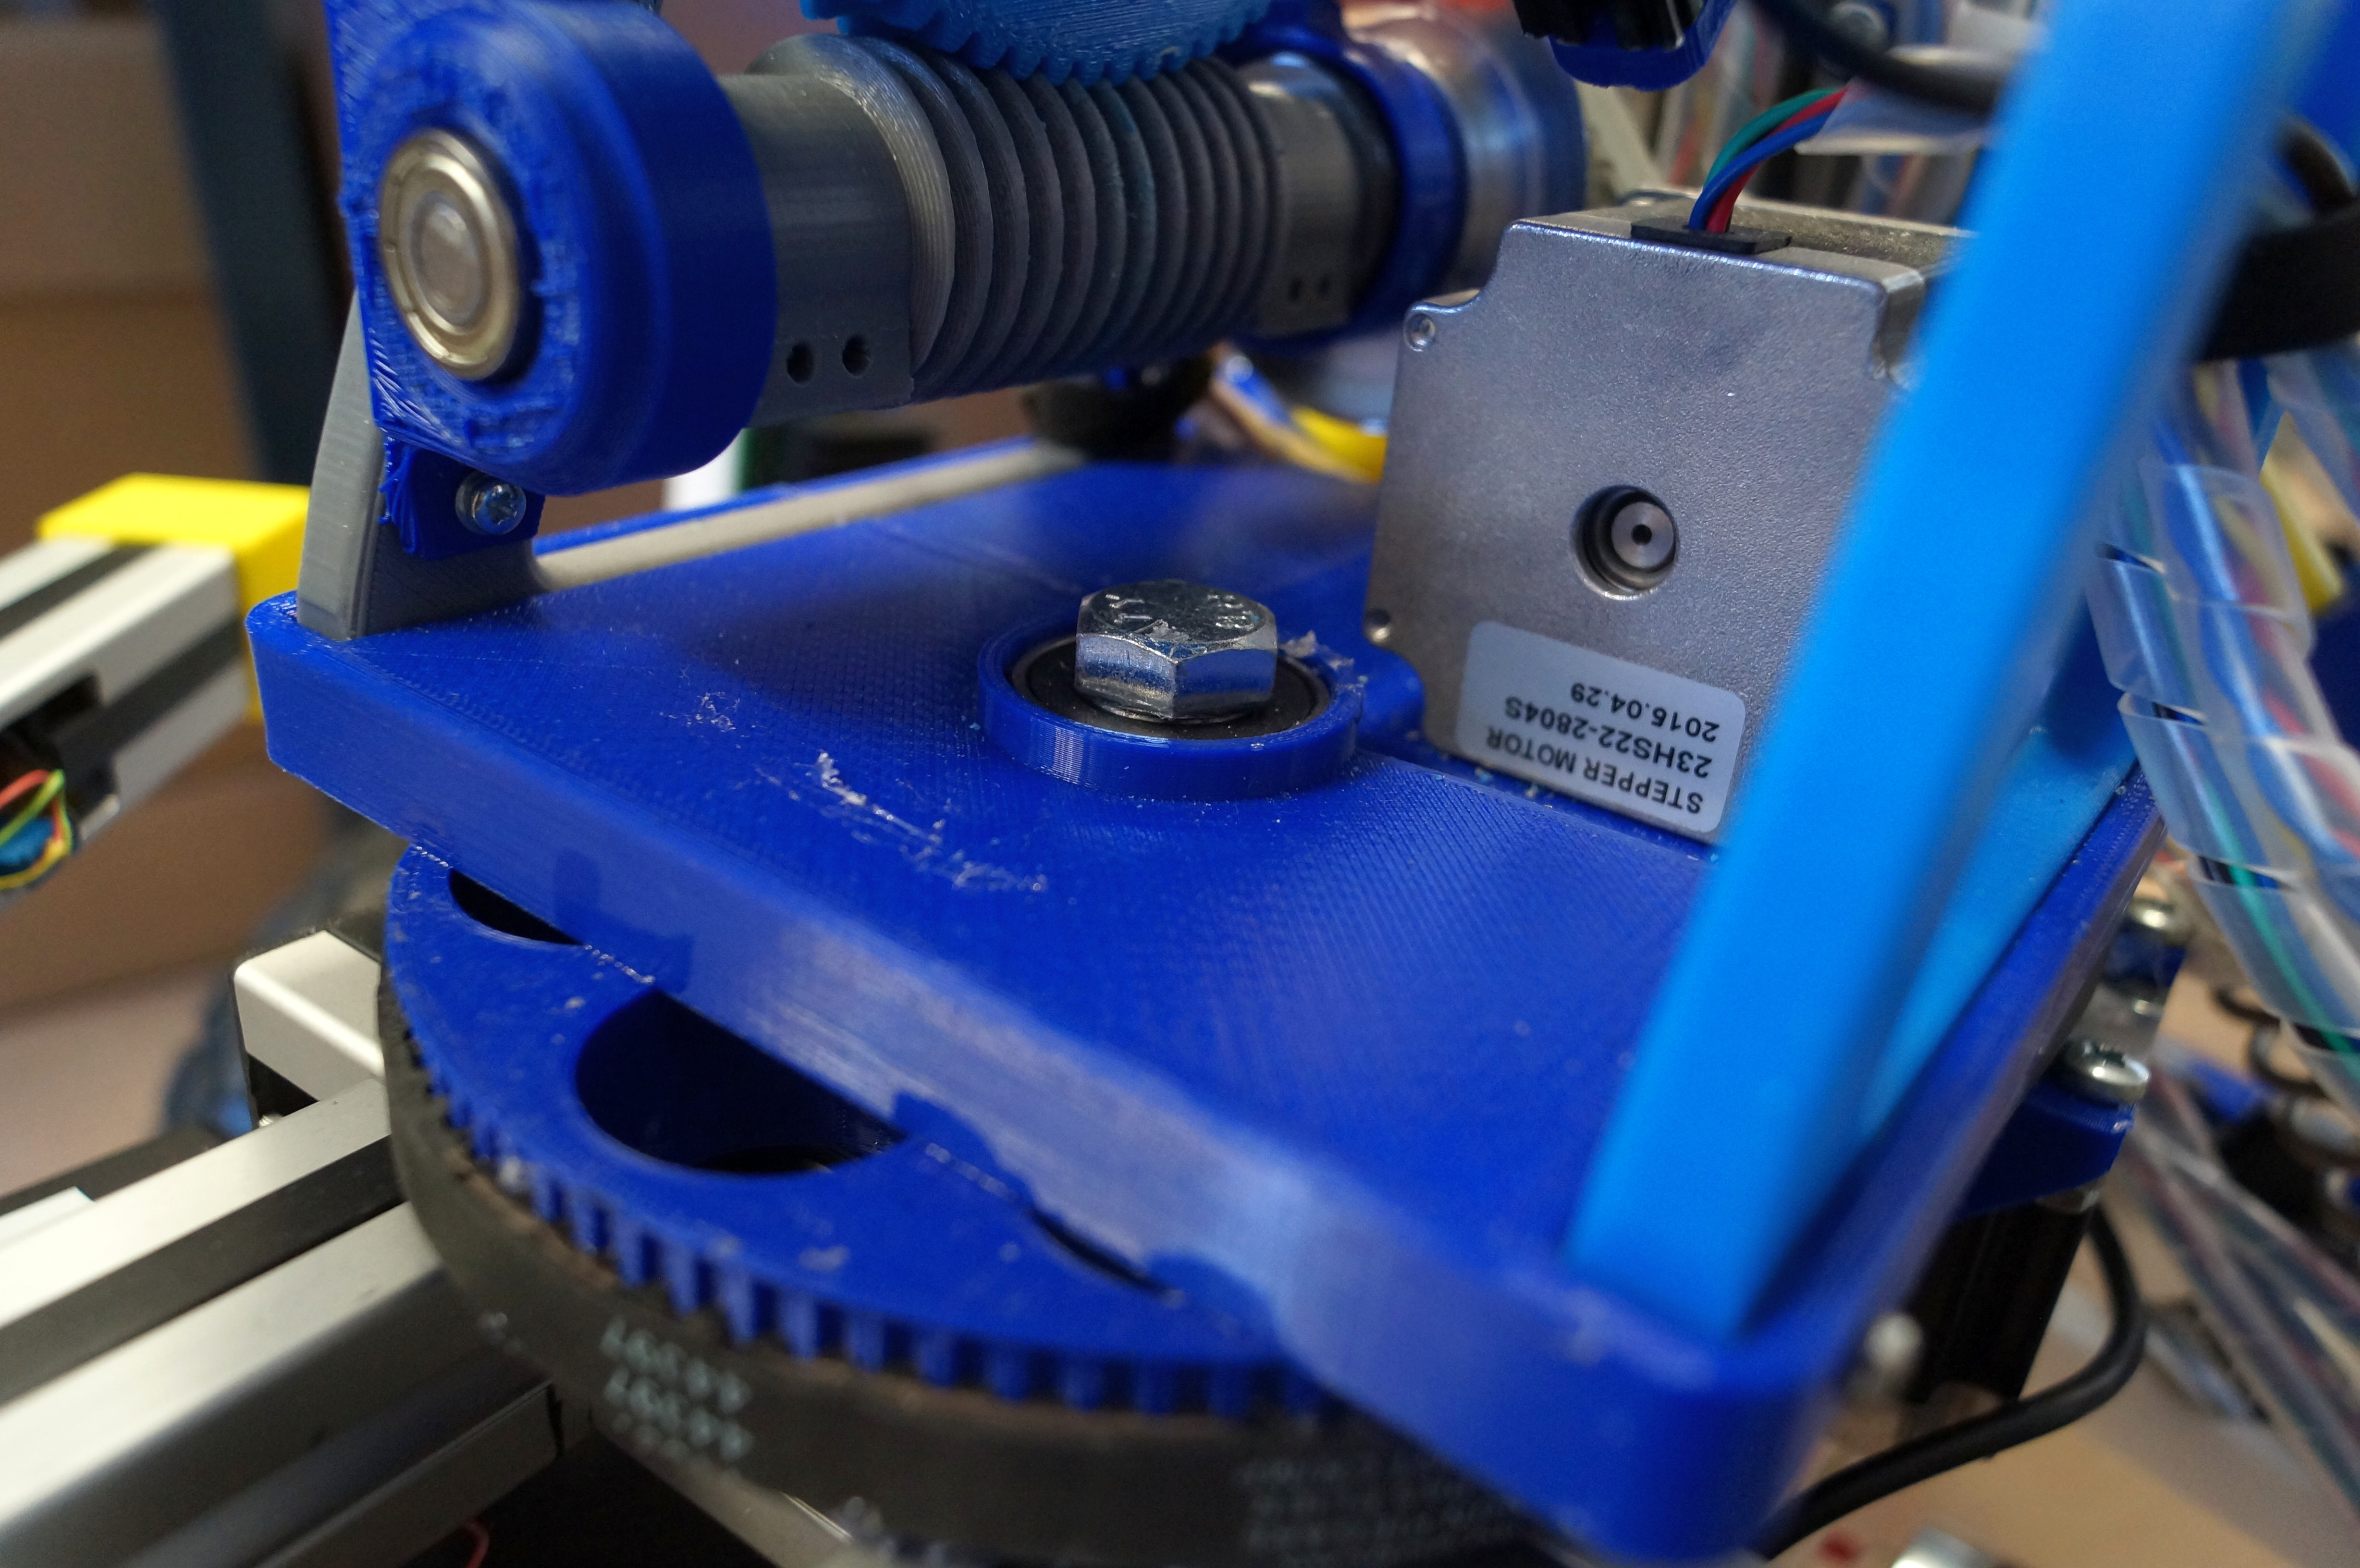
\includegraphics[width=10cm]{waist.jpg}
\end{center}
\caption{waist Joint}
\label{fig:waist}
\end{figure}

\subsubsection{Shoulder}
The shoulder joint controls the bottom part of the arm which holds the rest of the arm.  It is moved by a stepper motor connected to a corrugated rubber band in a similar fashion to the base.  The rubber band loops around a piece connected to a worm drive which rotates a large cog which sits at the base of the shoulder joint.  This enables the upper part of the arm to be moved to the correct altitude.  The arm is composed of two parallel thin pieces of aluminium extrusion with the wiring attached to the arm.  The joint of the waist to the shoulder is made with a specially designed 3D printed unit which holds both pieces of extrusion and has screws through two hold them tight as well as the aforementioned cog.  

\begin{figure}[!htb]
\begin{center}
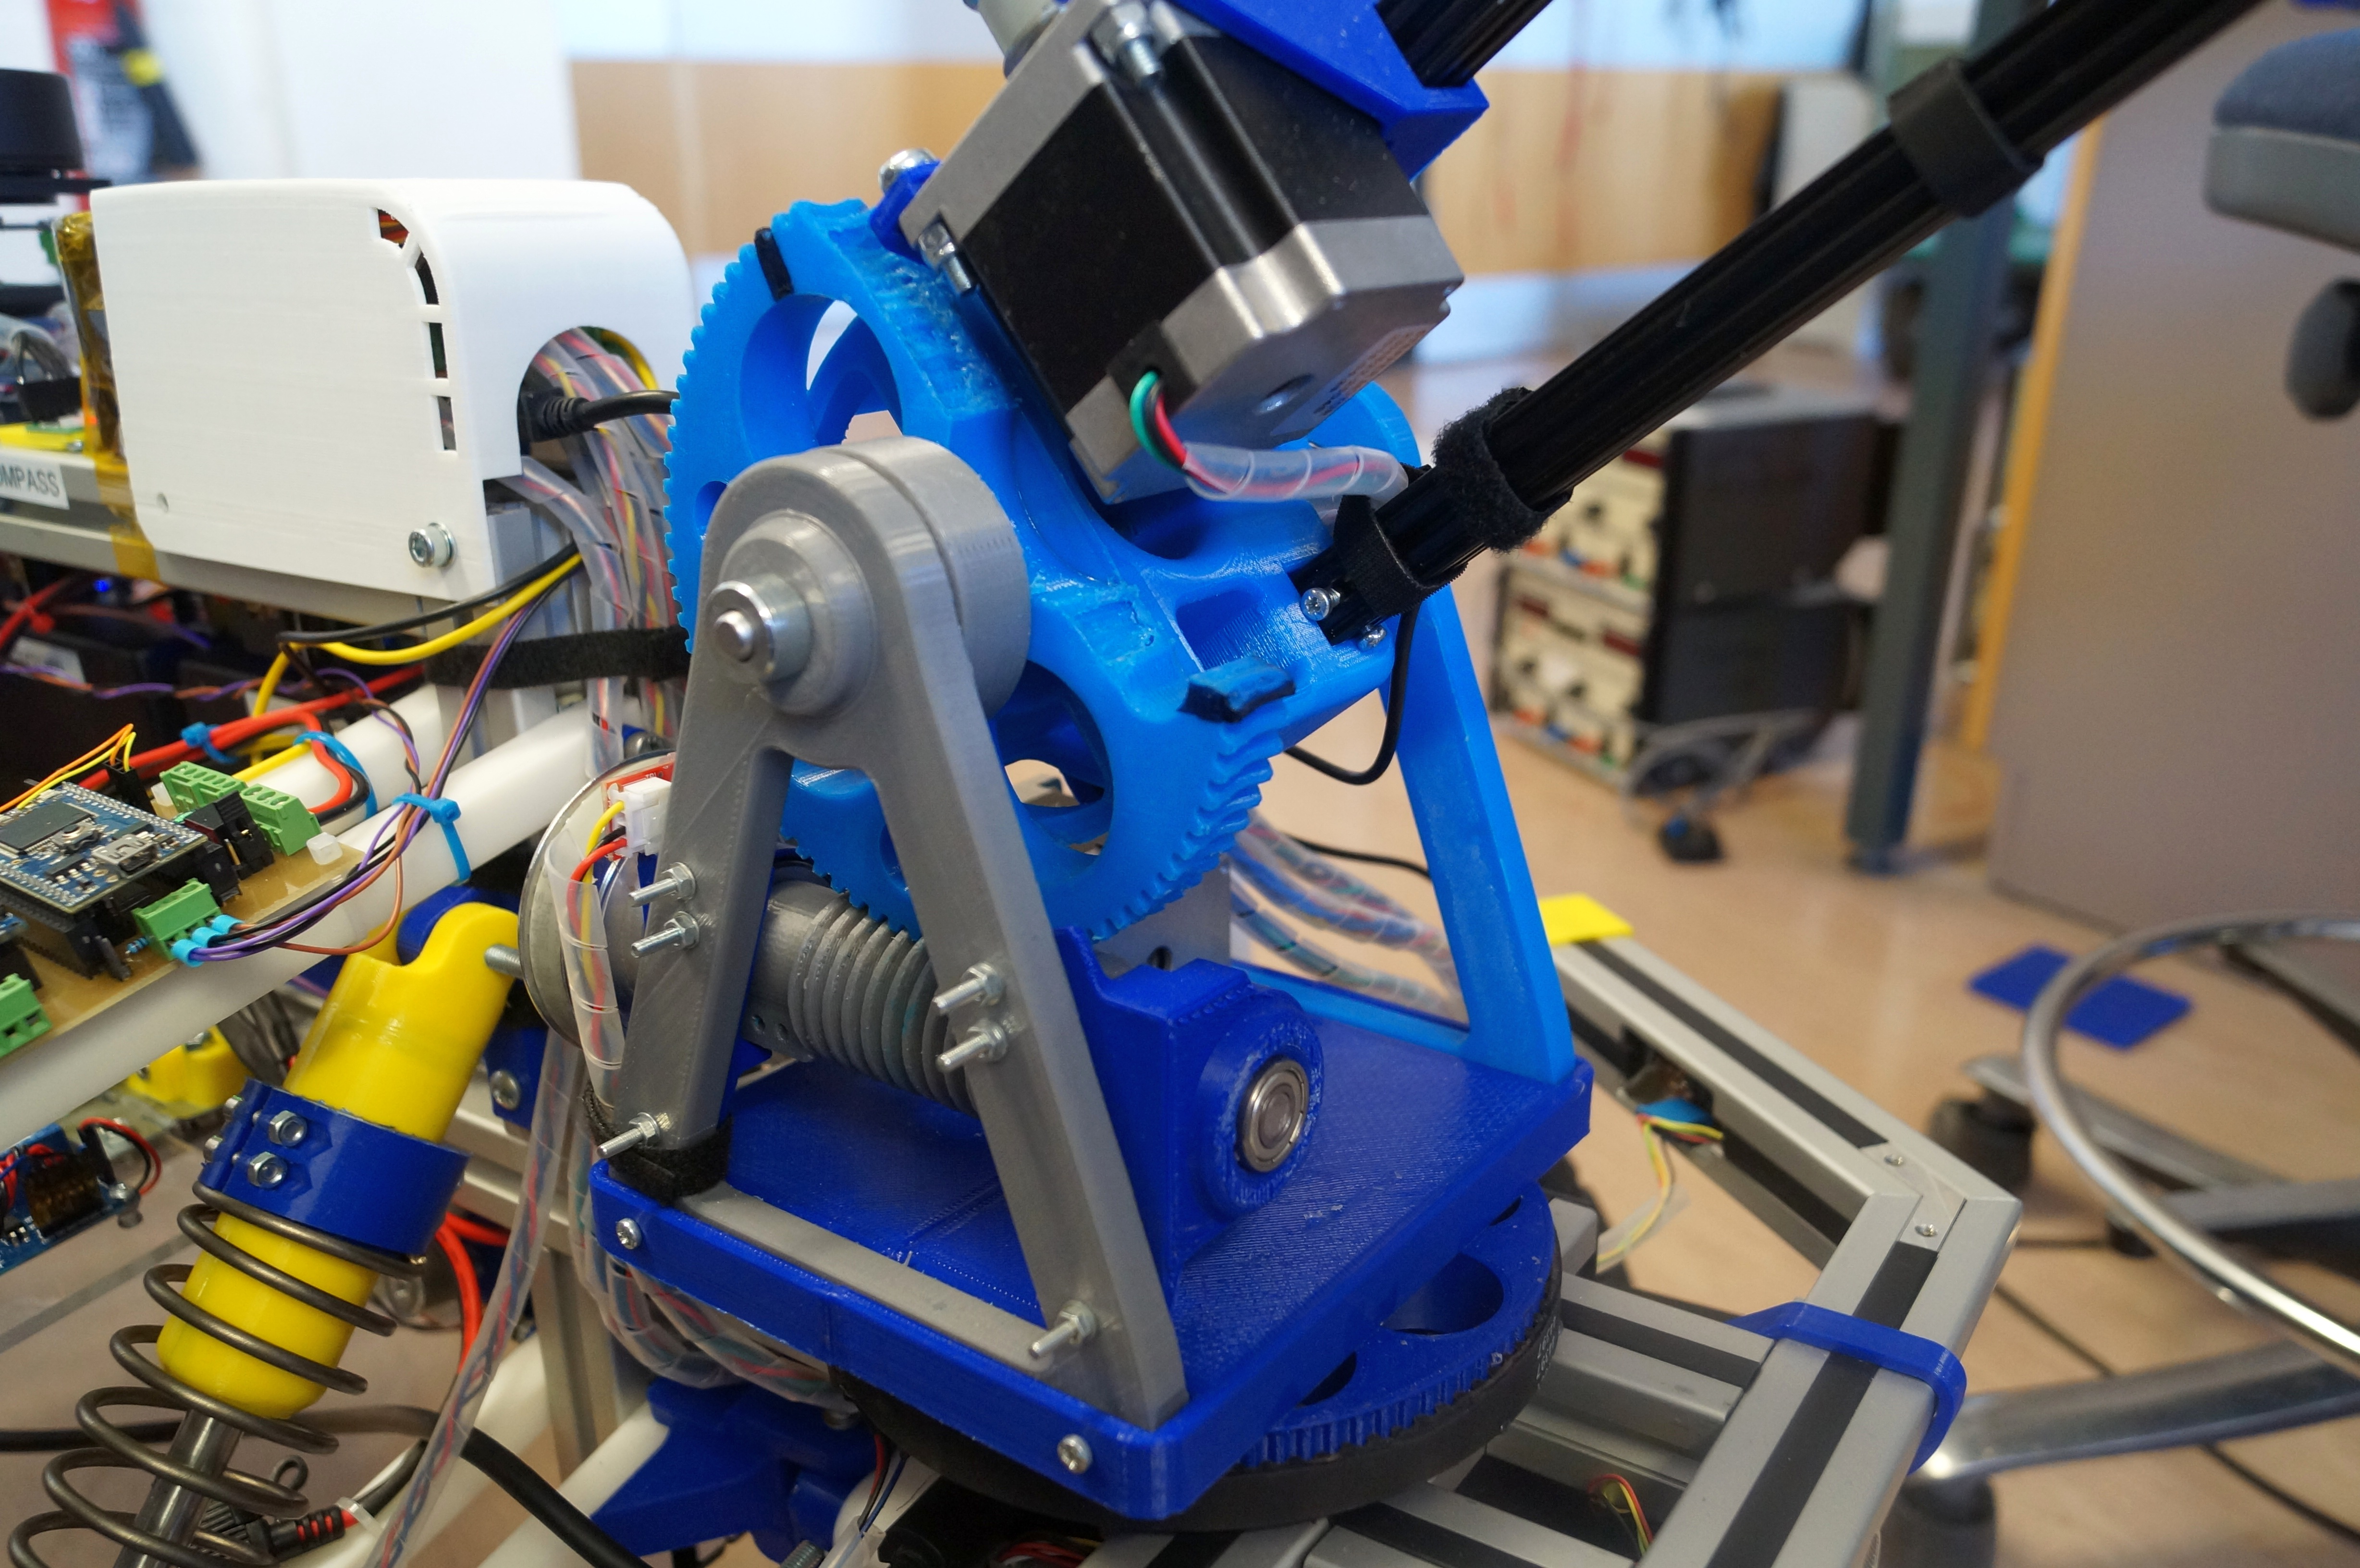
\includegraphics[width=10cm]{base.jpg}
\end{center}
\caption{Shoulder Joint}
\label{fig:shoulder}
\end{figure}

\subsubsection{Elbow}
The elbow section of the arm functions, and is constructed, in much the same way as the shoulder section.  Another stepper motor is attached near the base of the shoulder joint and directly turns a rubber belt which is connected to a worm drive which turns a cog connected to the upper arm segment.  The elbow joint is composed of two pieces of PLA which rotate freely around a metal bearing attached to a metal rod.

\begin{figure}[!htb]
\begin{center}
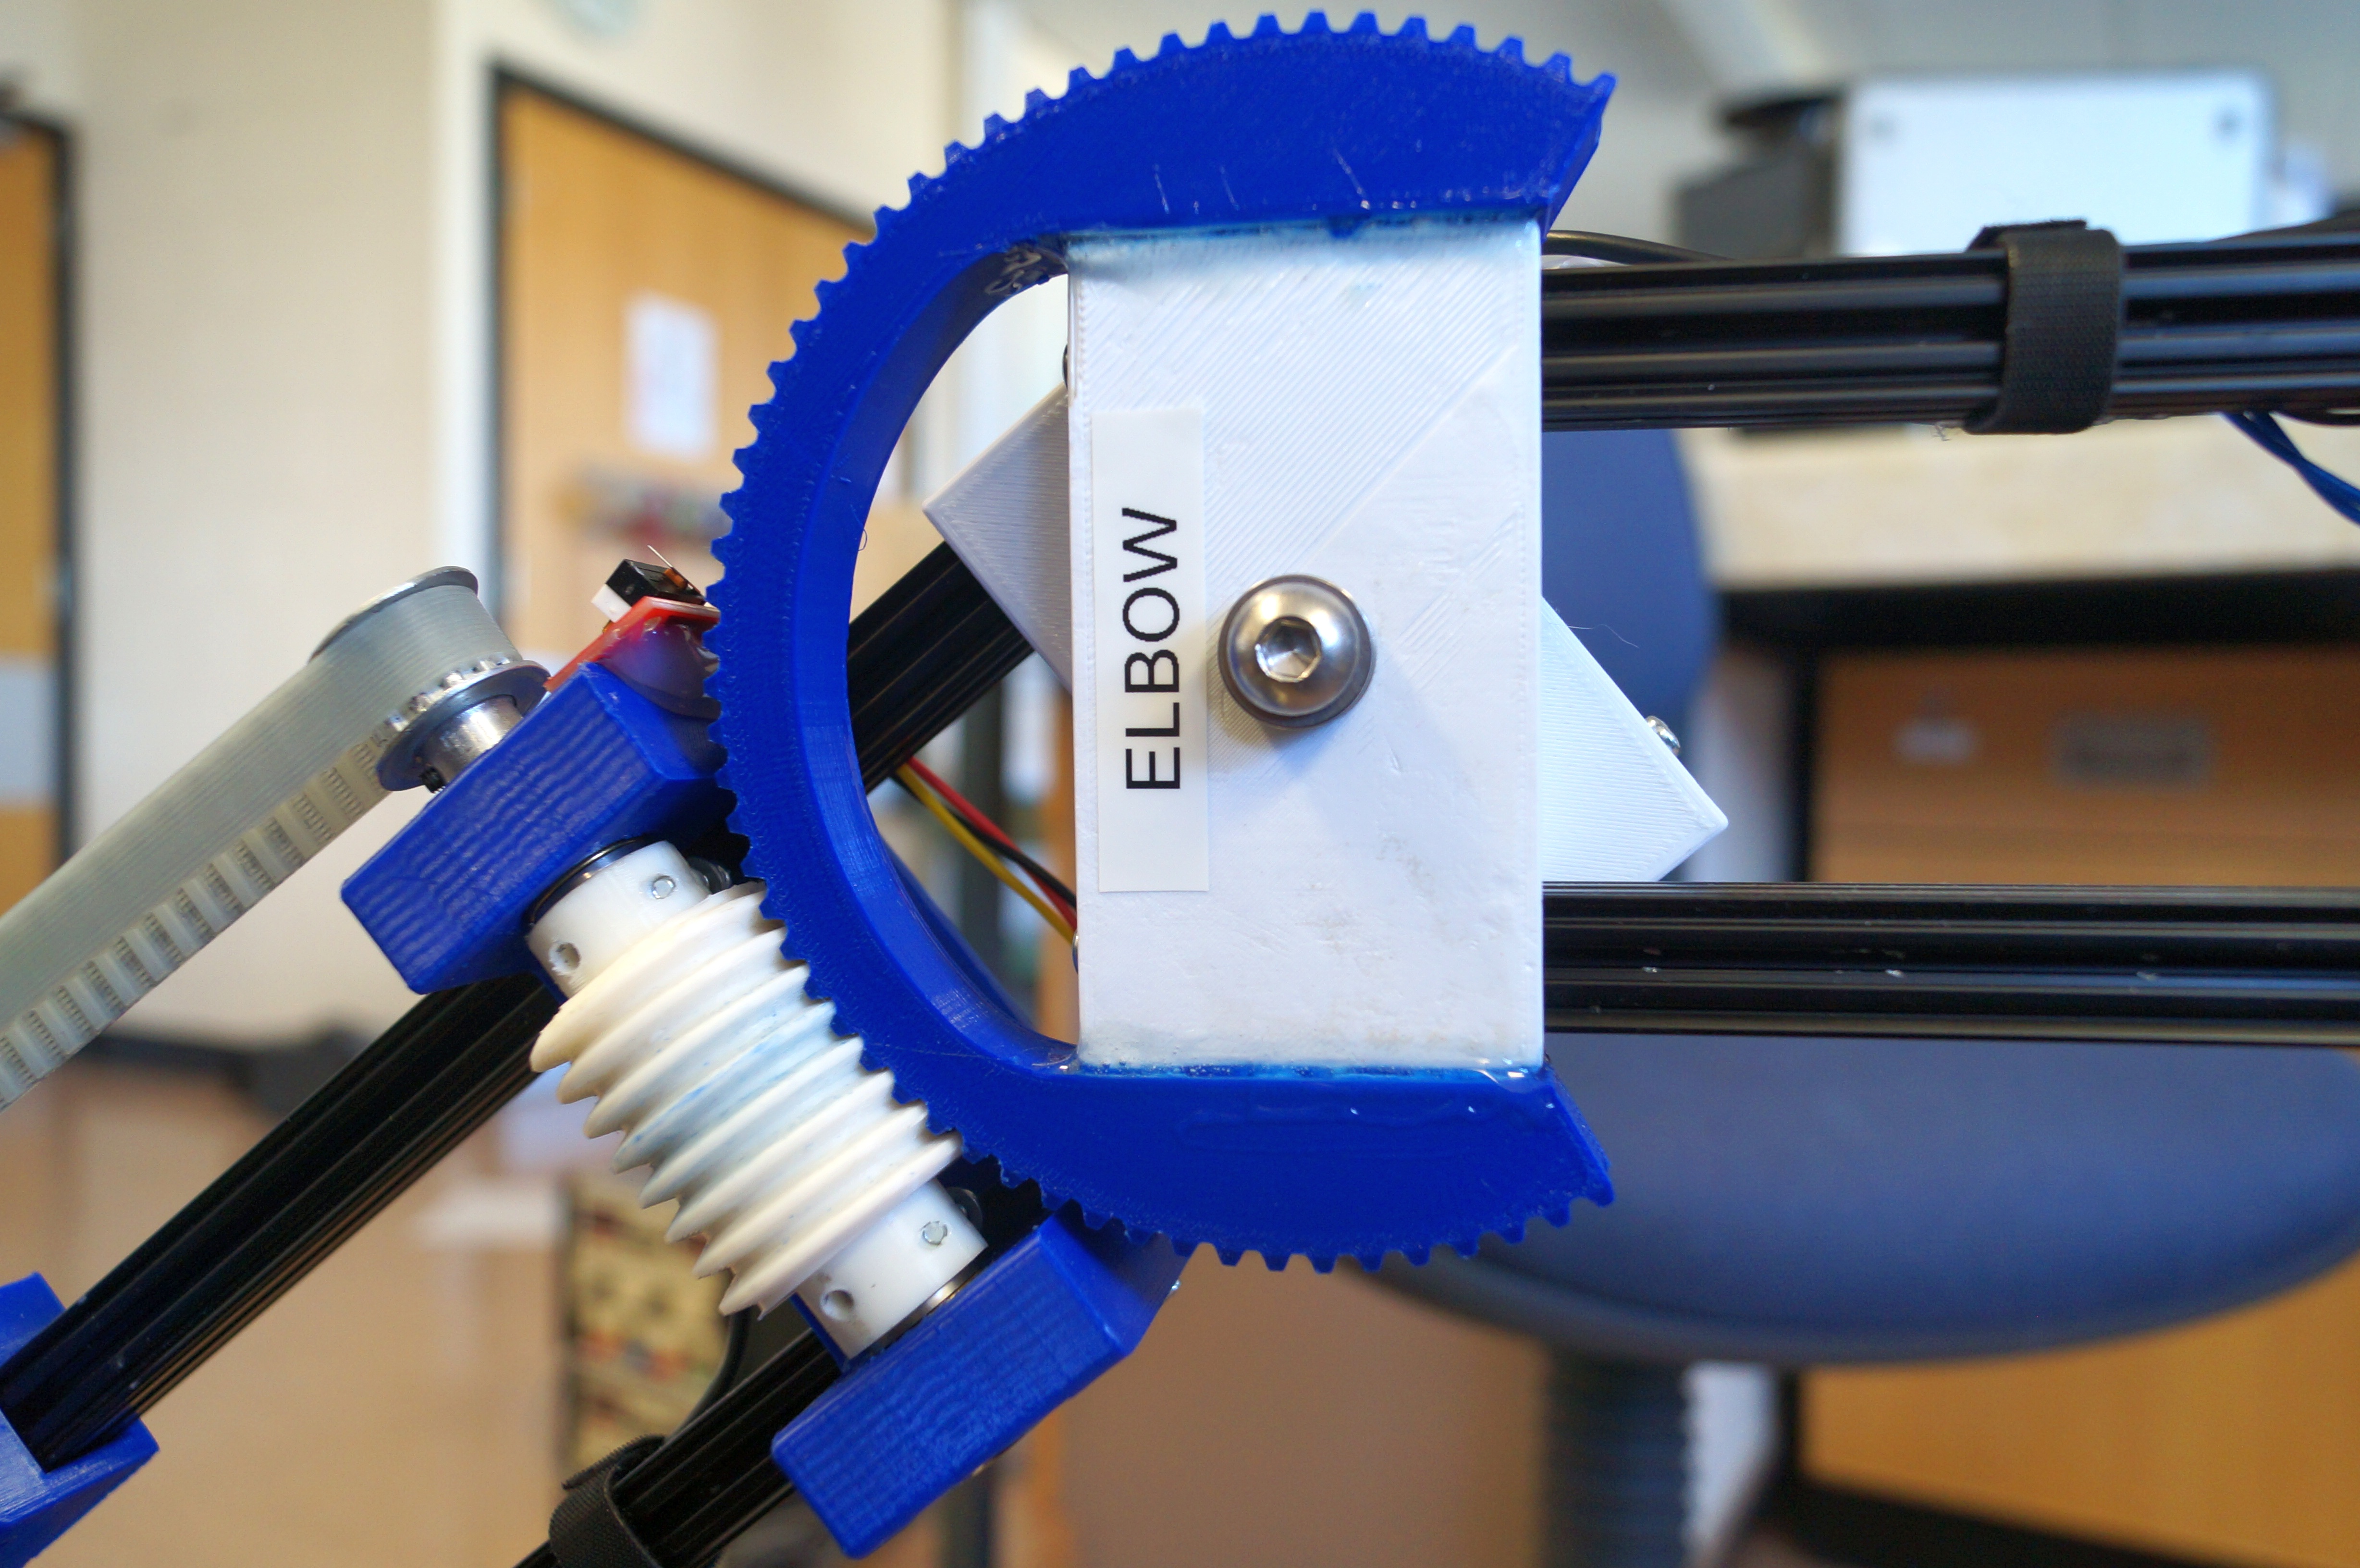
\includegraphics[width=10cm]{elbow.jpg}
\end{center}
\caption{Elbow Joint}
\label{fig:elbow}
\end{figure}

\subsubsection{Wrist}
The wrist section joins the upper arm with the gripper an has no motor control associated with it.  It was decided for simplicity to use a hanging gripper which acts due to gravity and would be able to dangle directly above an object before picking it up. 

\begin{figure}[!htb]
\begin{center}
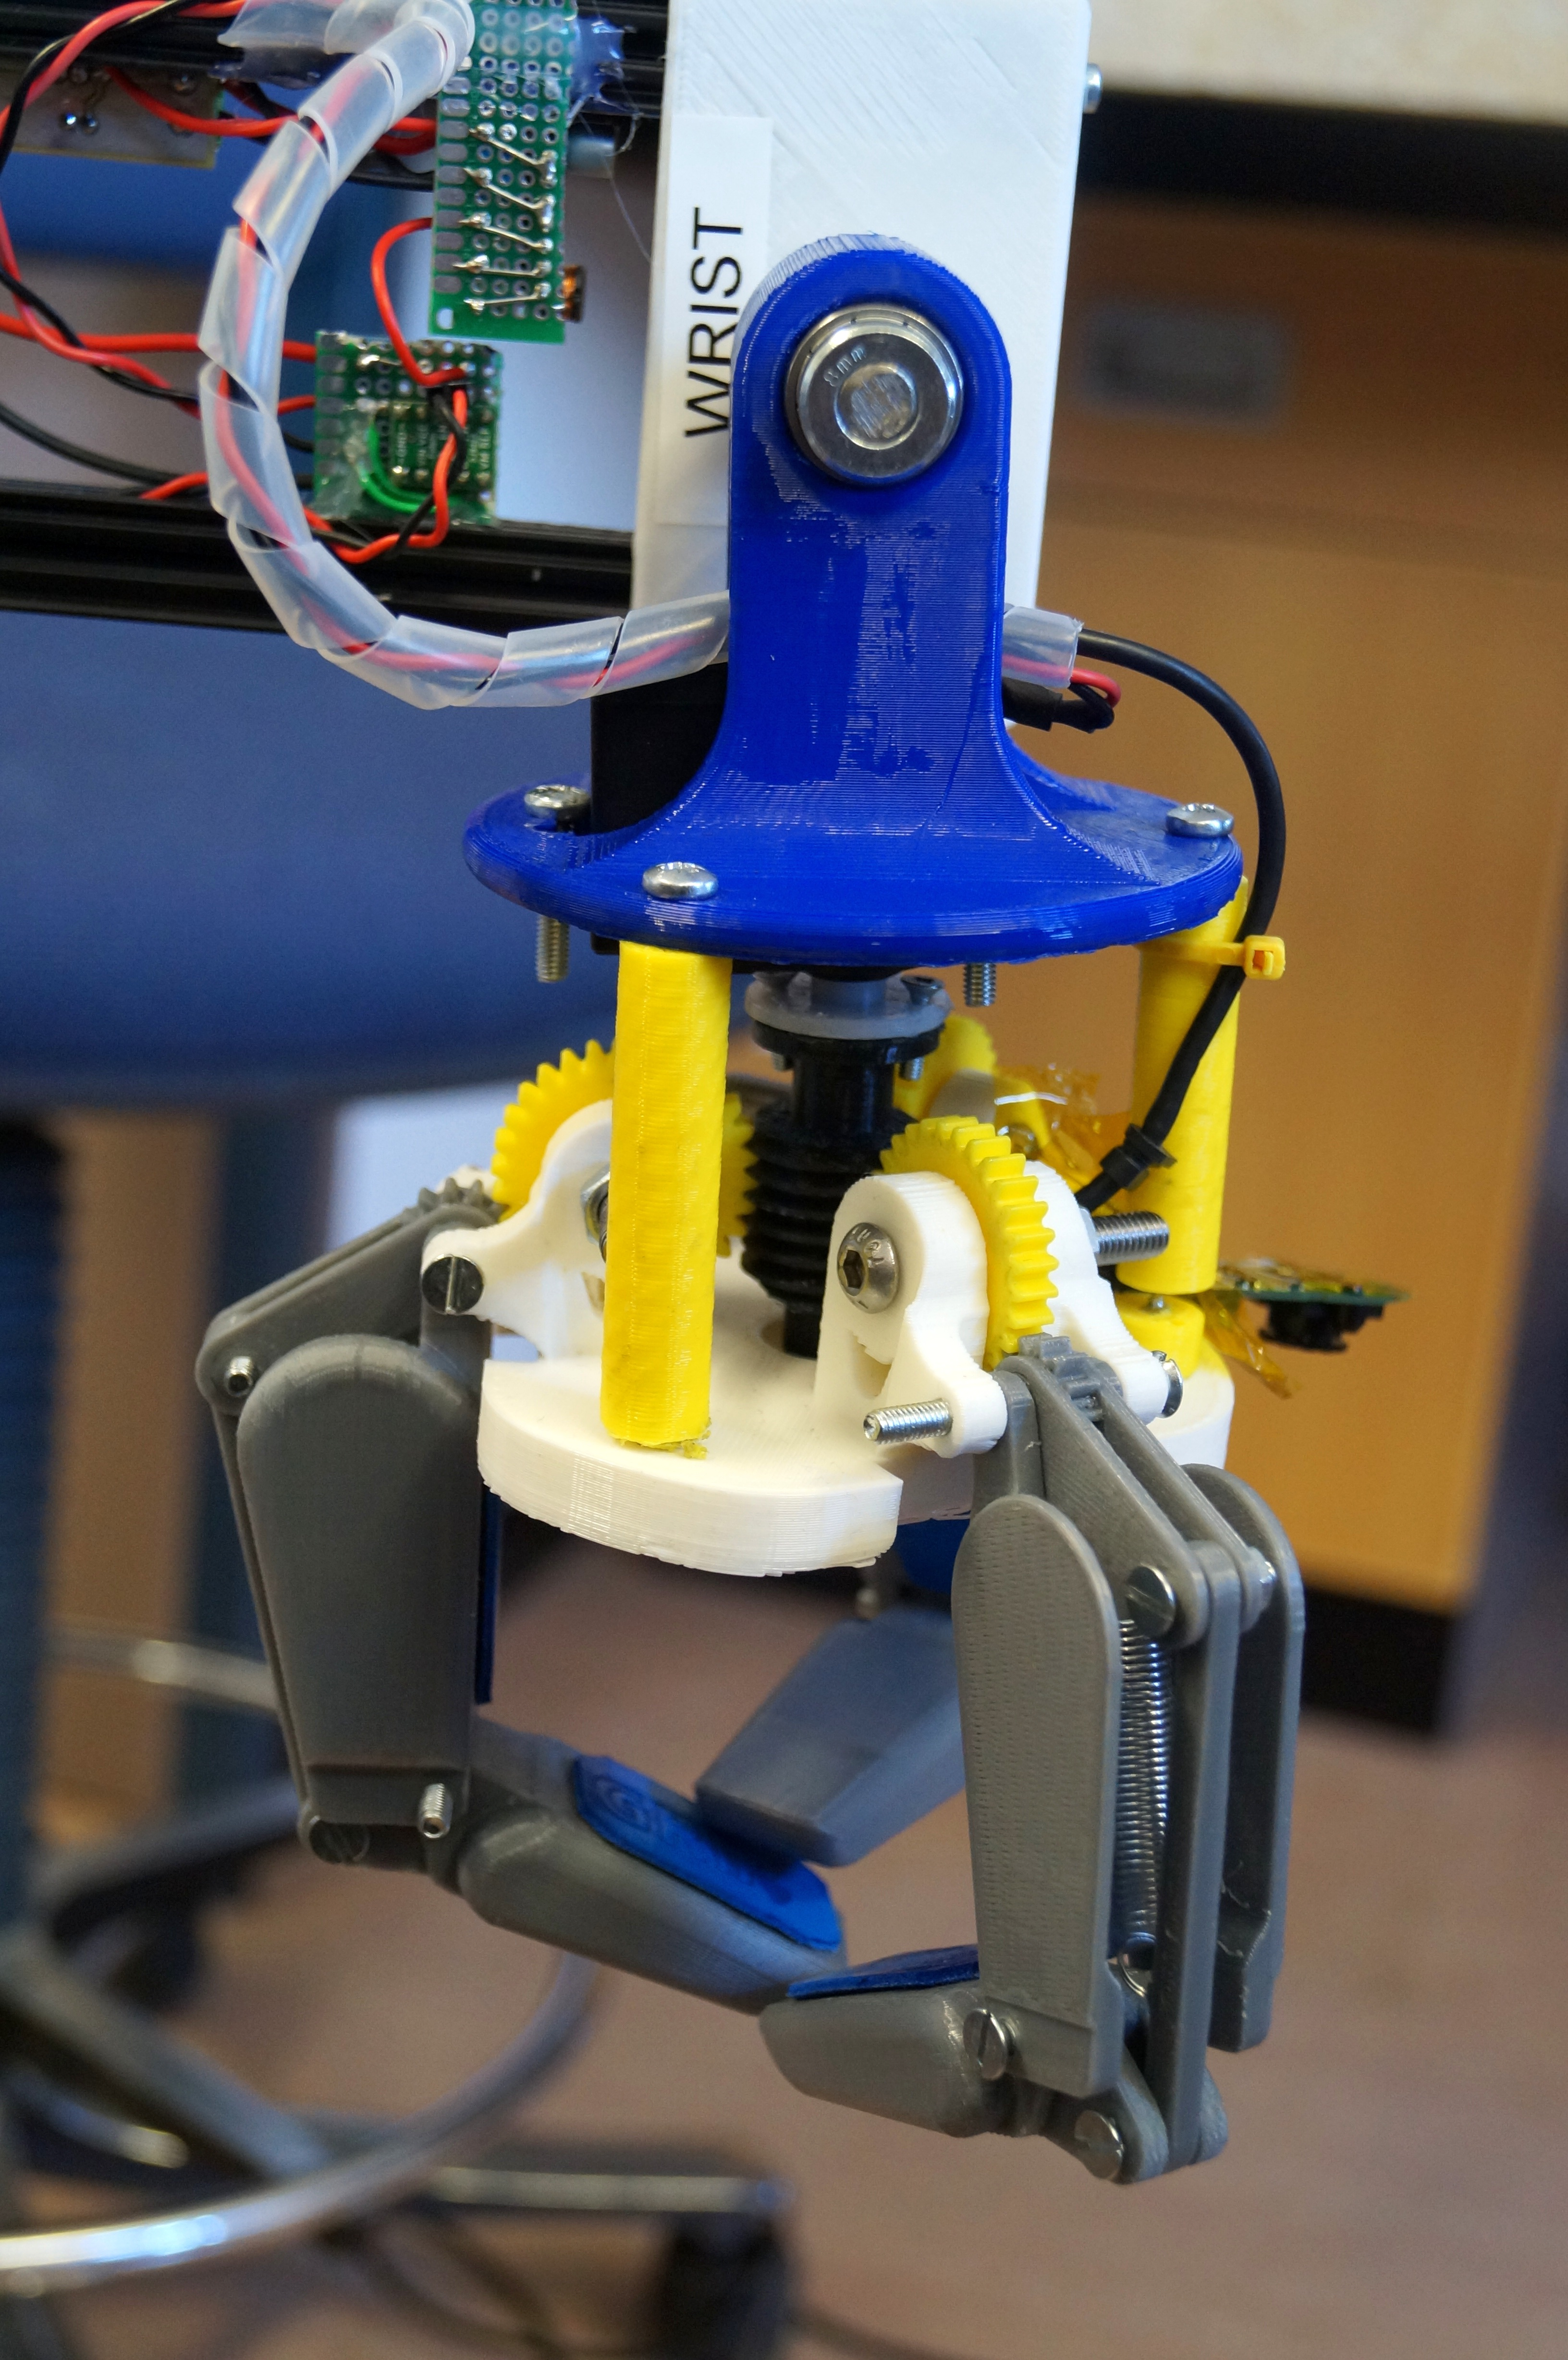
\includegraphics[width=10cm]{gripper.jpg}
\end{center}
\caption{Wrist Joint}
\label{fig:wrist}
\end{figure}

\subsubsection{End Effector}
The end effector (or gripper) was the hand-like device which hangs from the end of the upper arm.  It is the tool used to actually pick up objects and release them in the desired place (such as the proposed on board basket).  The gripper acted through the use of a servo.  A servo was stripped to function as a simple motor and this was given commands to either open or close for a set time.  This was done in 5 stages until fully open (homed position), or fully closed.  The stages of the grip are controlled by user input of a keyboard.

% * <em232@hw.ac.uk> 2016-05-09T08:52:06.770Z:
%
% > gripper printed...
% > \newline
% > Rubber strips were placed on the interior of the claws, to allow a strong grip on objects.
% > \newline
% > The webcam was situated inside the gripper. It was placed in the centre of the gripper, because its small size meant it would not impede any of the mechanics and also it makes picking up objects more intuative.
%
% ^.


\subsubsection{Electronics}
An Arduino Mega 2560 with a RAMPS1.4 shield was used to control the arm. A modified version of Marlin (3d printer firmware) was used. This handled homing and moving to positions in joint space. Python code was written to interface with the firmware using G-Code  (RS-274 numerical control programming language) 

\subsubsection{Materials}
The arm was constructed using several different materials. The main load bearing beams use openbeam aluminium extrusion. PLA was used for all printed parts except the worm gear in the gripper which was printed in nylon 6.

\subsubsection{Parking} \label{parking}
The arm was designed to pick up objects and then put them into a basket and return to the park position so that Tiberius could continue on its mission unimpeded. This was chosen to be at an acute angle close to the back right wheel.

\subsubsection{Homing}
As discussed in \textit{Parking} \ref{parking} the arm will always start from the same location. This makes the task of homing relatively easy since we know where the arm will start. It was decided that the arm should home backwards which meant it would flip to a position at the front of Tiberius. The arm then moves to its centre location in front of Tiberius. 



\subsection{Software Design}
The main control code of the arm is designed to stop it from damaging itself or Tiberius. With allowed angles for each joint and position in Cartesian space defined. Assuming that the arm thinks it is in the correct location.

\subsubsection{Inverse Kinematics}

This involved taking a 3 dimensional Cartesian coordinate and converting it into angular coordinates that the three arm joints would position to.  The basic way this was done was by using trigonometry to identify the required rotation angle, which would be done with the waist joint and by using further trigonometry to determine the two joint angles required to manoeuvre the joints to the correct point in space.	

The code was designed to be flexible and adaptable so the arm segments’ lengths were used as parameters in the code along with the x, y and z Cartesian coordinates of the desired position.  

Each Cartesian coordinate was converted into the angles of the three motors from rest, which were denoted as ρ,σ and τ.  The angle of rotation, ρ around the base of the arm, was controlled by a large stepper motor, τ was the angle of the upper arm joint which could be positioned forwards or backwards depending on the depth of the object being picked up and σ was the angle of the elbow joint which allowed the gripper to be positioned above the object of interest.  

\begin{figure}[!htb]
\begin{center}
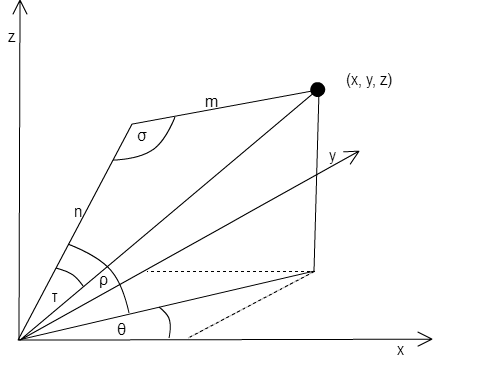
\includegraphics[width=15cm]{Cartesian2.png}
\end{center}
\caption{Transformation from Cartesian Coordinates}
\label{fig:cartesian}
\end{figure}

\begin{capequ}[!htb]
\begin{center}
\begin{equation}
\cos \tau = \frac{m^{2}+s^{2}-n^{2}}{2ms}
\end{equation}
\label{Equation1}
\end{center}
\end{capequ}

\begin{capequ}[!htb]
\begin{center}
\begin{equation}
\cos \sigma  = \frac{m^{2}+n^{2}-s^{2}}{2mn}
\end{equation}
\label{Equation2}
\end{center}
\end{capequ}

\begin{capequ}[!htb]
\begin{center}
\begin{equation}
\tau = cos^{-1}\left (\frac{m^{2}+s^{2}-n^{2}}{2ms}\right )
\end{equation}
\caption{}
\label{Equation6}
\end{center}
\end{capequ}

\begin{capequ}[!htb]
\begin{center}
\begin{equation}
\rho = tan^{-1}\left ( \frac{z}{\sqrt{{x^{2}+y^{2}}}} \right )+ cos^{-1}\left ( \frac{m^{2}+(x^{2}+y^{2}+z^{2})}{2mn} \right )
\end{equation}
\caption{Elevation Angle of Upper Arm}
\label{Equation3}
\end{center}
\end{capequ}

\begin{capequ}[!htb]
\begin{center}
\begin{equation}
\theta = tan^{-1}\left (  \frac{y}{x}\right )
\end{equation}
\caption{Rotation Angle of Base}
\label{Equation4}
\end{center}
\end{capequ}

\begin{capequ}[!htb]
\begin{center}
\begin{equation}
\sigma = cos^{-1}\left (\frac{m^{2}+s^{2}-(x^{2}+y^{2}+z^{2})}{2ms} \right )
\end{equation}
\caption{Elbow Joint Angle}
\label{Equation5}
\end{center}
\end{capequ}

\subsubsection{Safety}
There were a few considerations when dealing with the operation of the arm.  Firstly the use of several motors and a fair amount of current meant that they had to be safely electrically insulated.
Another feature was that the arm could potentially swing around and damage the rest of Tiberius so precautions had to be made with end point switches and careful parameters in the code to prevent the arm moving beyond certain bounds.

\subsubsection{Manual control}
The ability to manually control the arm was necessary as the...The arm can be controlled with simple keyboard presses for up/down, left/right an back/forward.
This moves the arm in increments for every command in that direction.

\subsubsection{Camera}
The gripper had a small web cam attached so that the user could see what is being picked up.
This enabled remote control of the arm through the web interface in real time.
